\chapter{Installing Twiz O' Meter on Your Car}

Installing ToM+ on your Twizy is actually really simple and doesn't need any special
knowledge since, as I usually say, it's a “plug and drive” device! So follow this few
steps to correctly and quickly install it or try on your own a different location.

\section{Display LCD position}

When ordering the device, you can choose to have the 3D stand along with the clip-on display.
So you can choose to install the display in two different ways: using the clip-on mode or
using the 3D stand mode. The clip-on mode is the most common and it allows you to attach the
display to the car's dashboard, while the 3D stand mode allows you to place the display on 
a flat surface inside the car (I usually suggest the right or left glove box).

\subsection{Clip-on mode}

If you choose this mode, it is really simple. You just need to clip the display on the 
dashboard, in a position that is comfortable for you to see while driving. Put the top
part of the display on the dashboard and then push the bottom part until it clicks in place.

\begin{figure}[H]
    \centering
    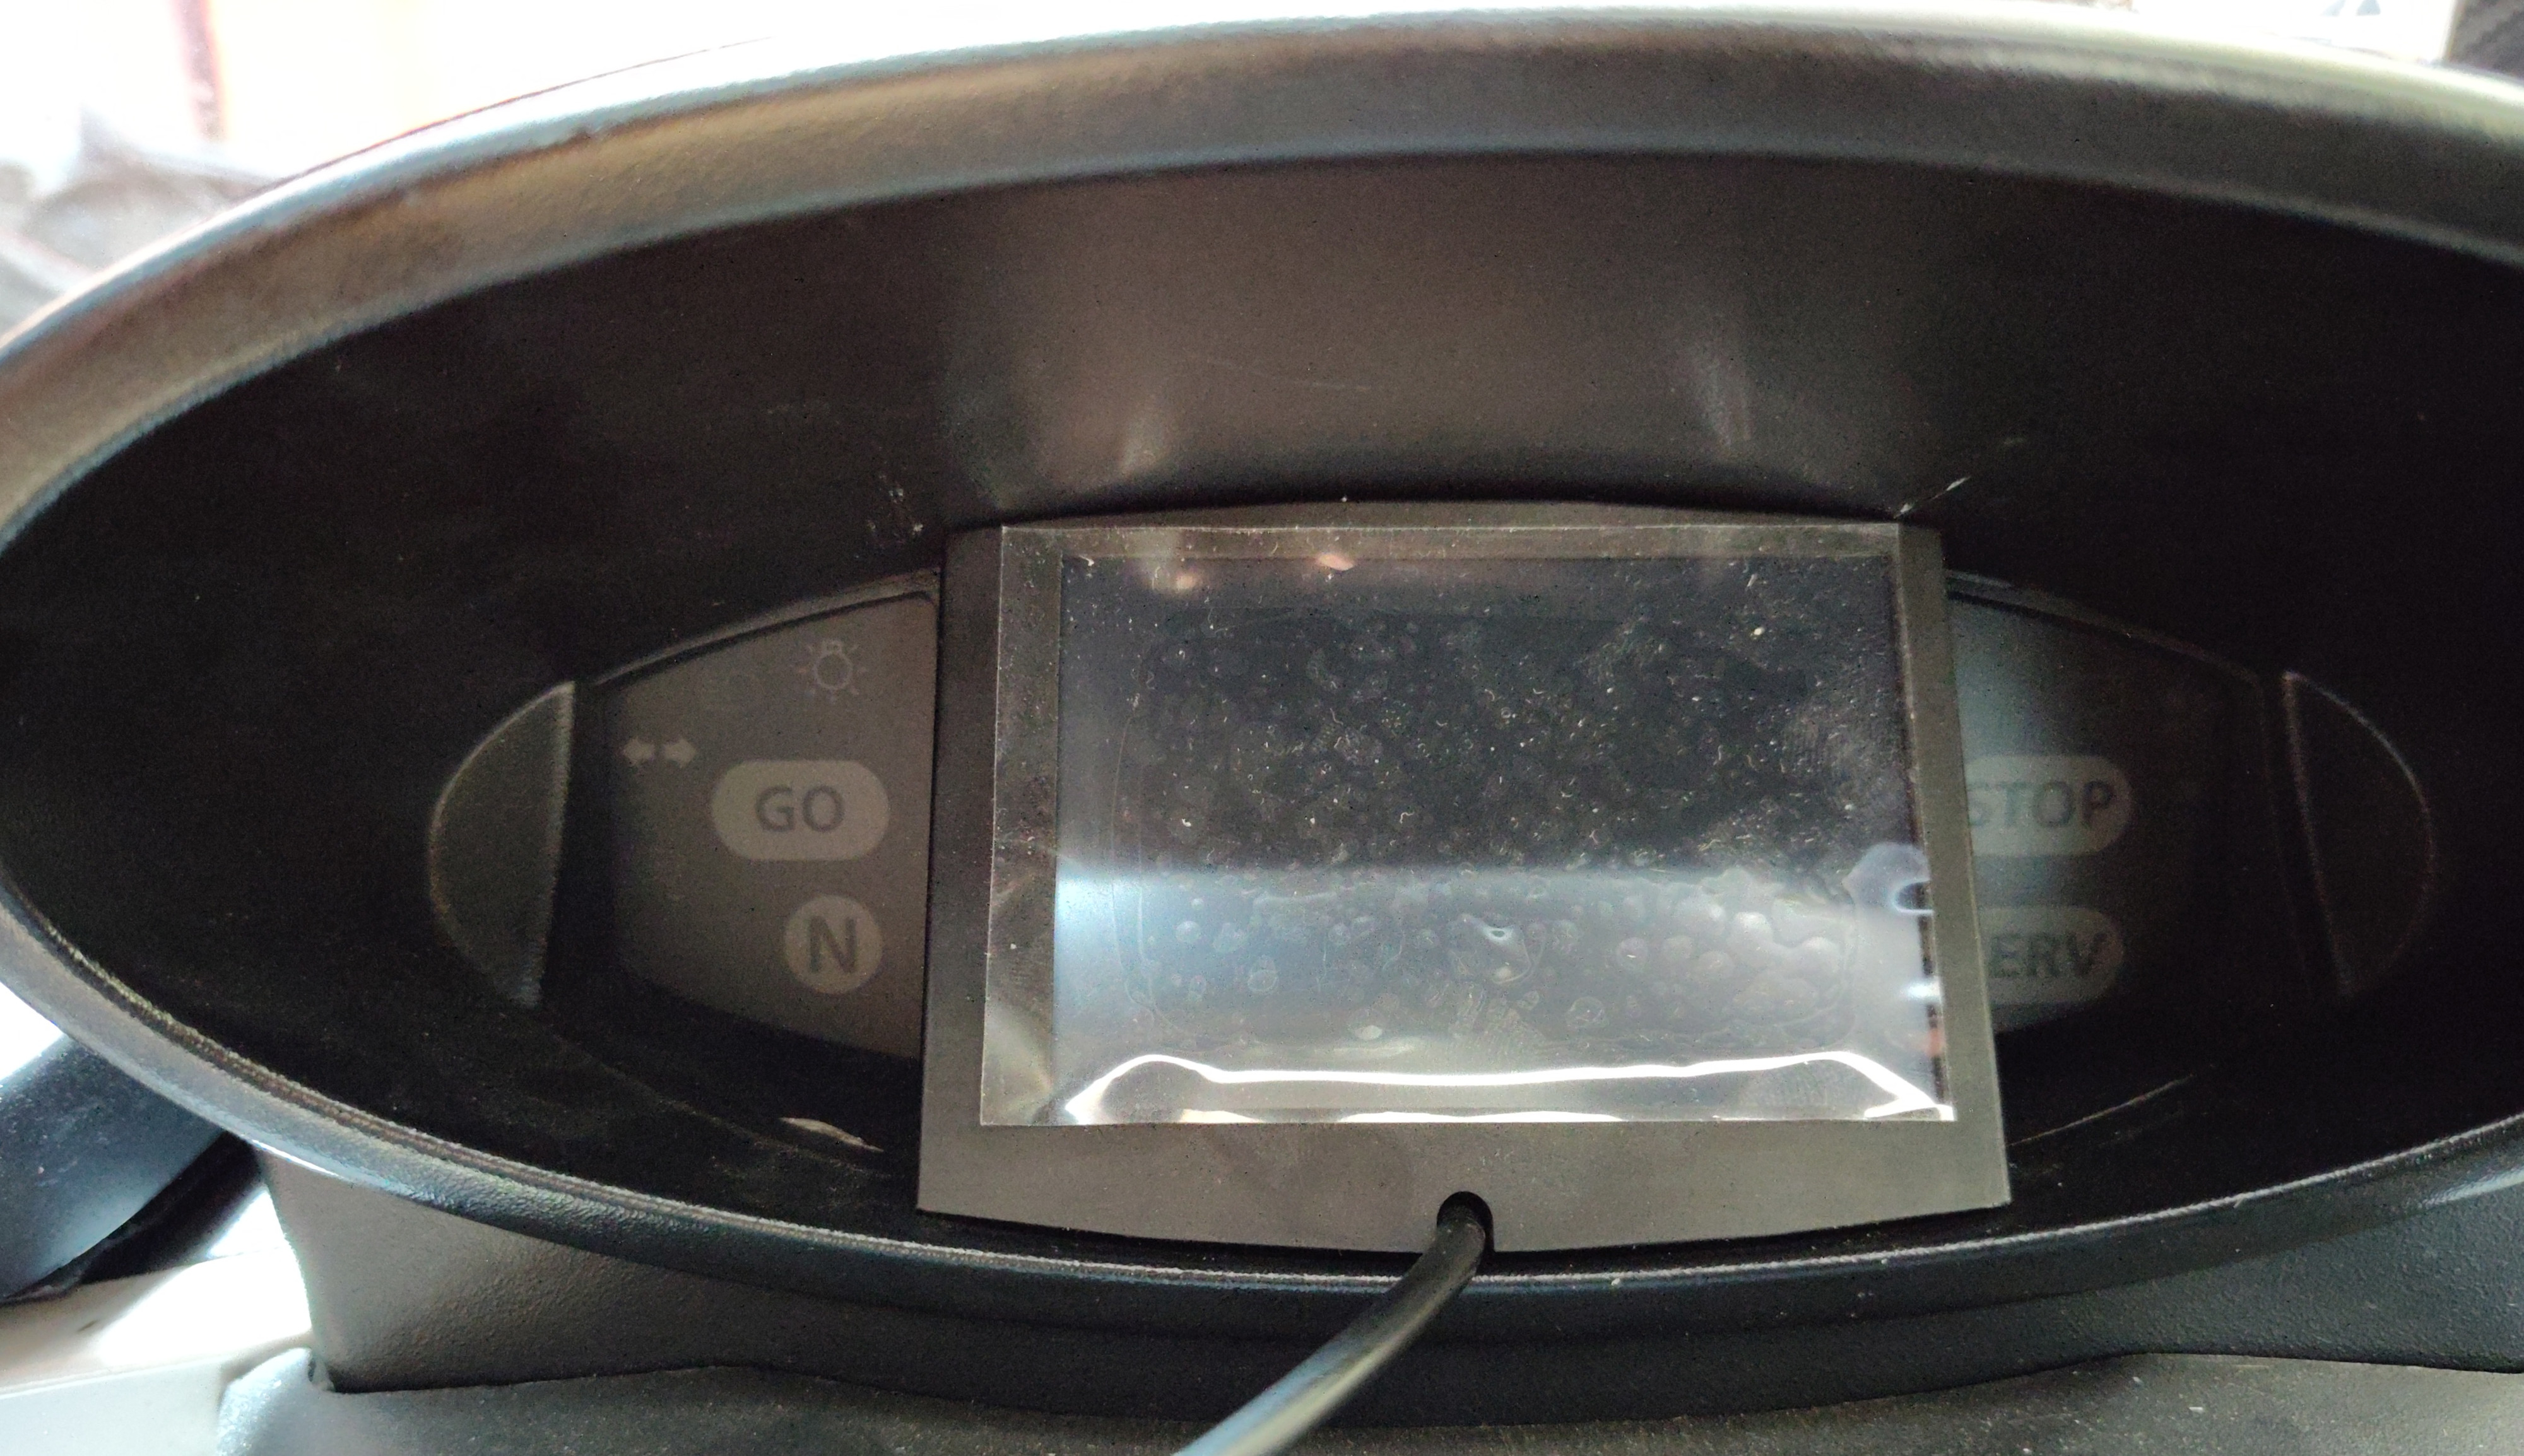
\includegraphics[width=0.8\textwidth]{figures/clip_on.jpg}
    \caption{Clip-on mode installation}
\end{figure}

Make sure that the cable is not pinched in the bottom part of the display but it is free
to move in the apposite hole, otherwise you might damage the cable. Then remove
the protective film, if you want.

\subsection{3D stand mode}

If provided, you can use the 3D stand to place the display on a flat surface inside the car.
You can put a double-sided tape on the bottom, so you can stick it to the surface.
Or you can use the screwholes on the bottom of the stand to fix it with two screws.

As we did for the clip-on mode, make sure that the cable is not pinched in the back part of the display
when putting the cover on but it is free to move in the apposite hole, otherwise you might damage the cable.
Refer to Figure~\ref{fig:back_cover} and Figure~\ref{fig:bottom_cover_screwholes} at page~\pageref{fig:back_cover} to see the mentioned parts.
This is how the 3D stands looks without the display installed.

\begin{figure}[H]
    \centering
    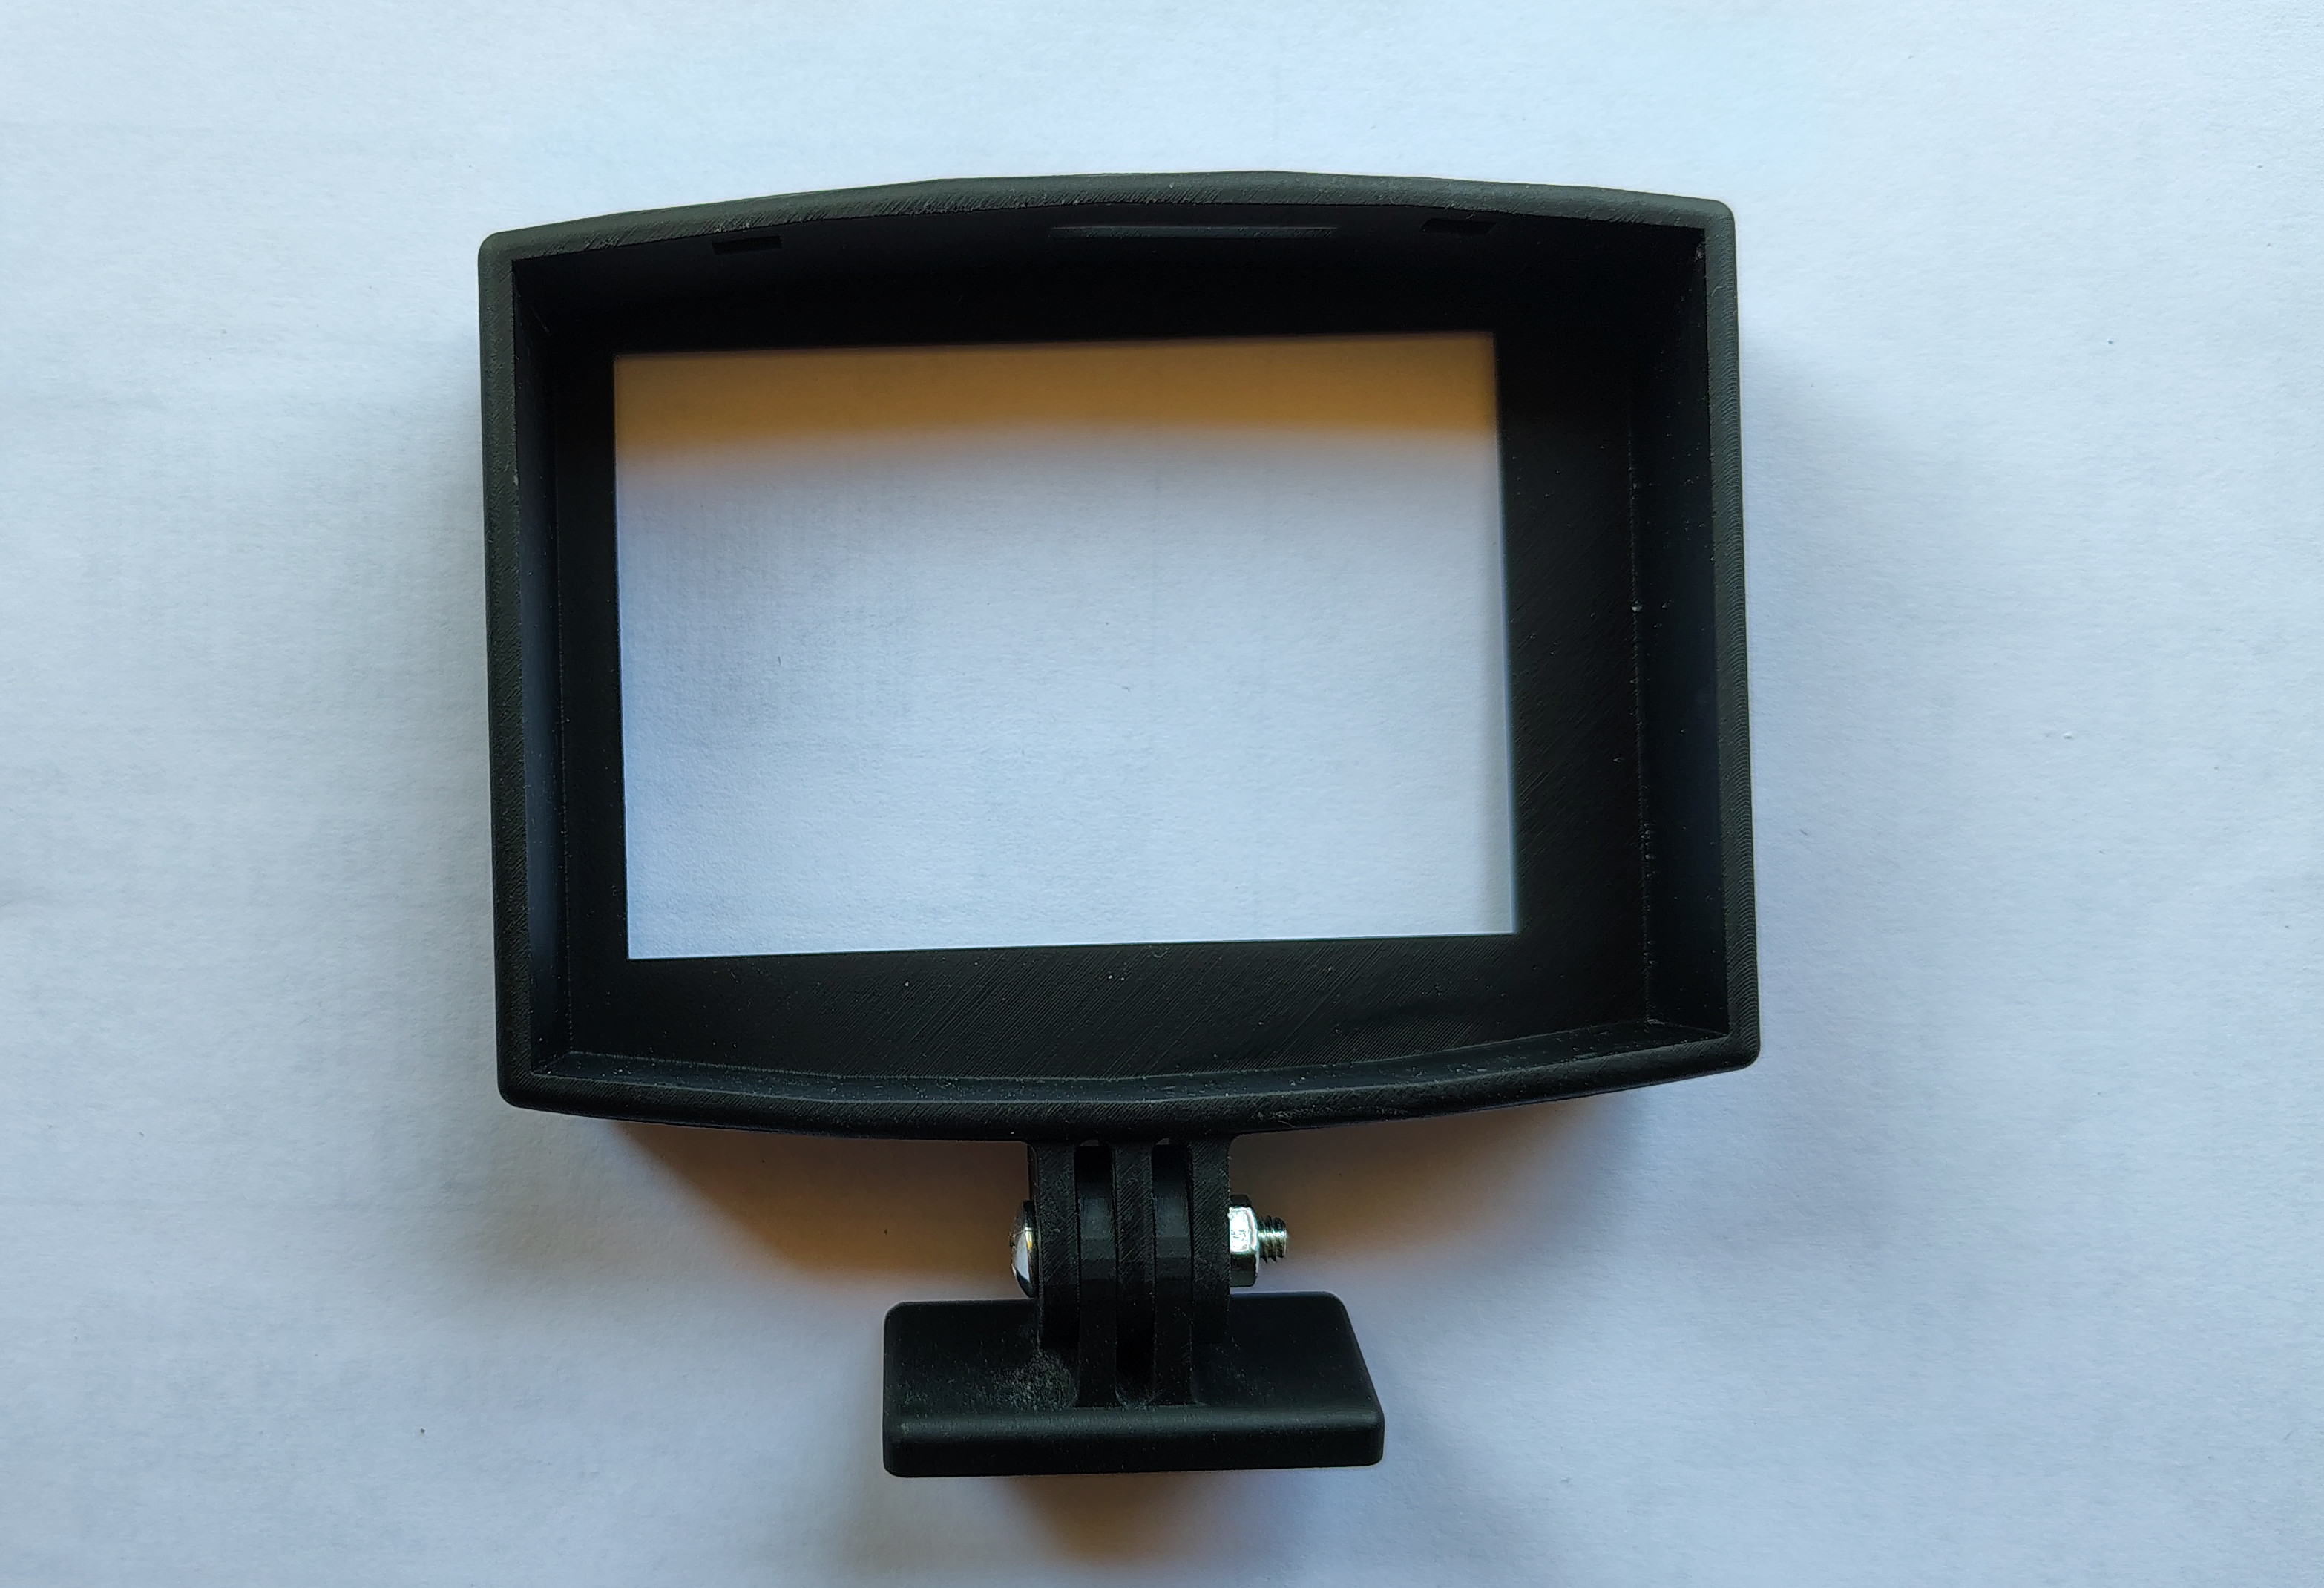
\includegraphics[width=0.8\textwidth]{figures/3d_stand.jpg}
    \caption{3D printed empty stand}
\end{figure}

\subsection{Cable connection}

Then you can remove the protective film from the display and plug in the cable to power it.
The other end of the cable needs to be connected to the black box, which will be installed in the next step.
It fits only in one way, so make sure to align the connector properly before plugging it in.

\begin{figure}[H]
    \centering
    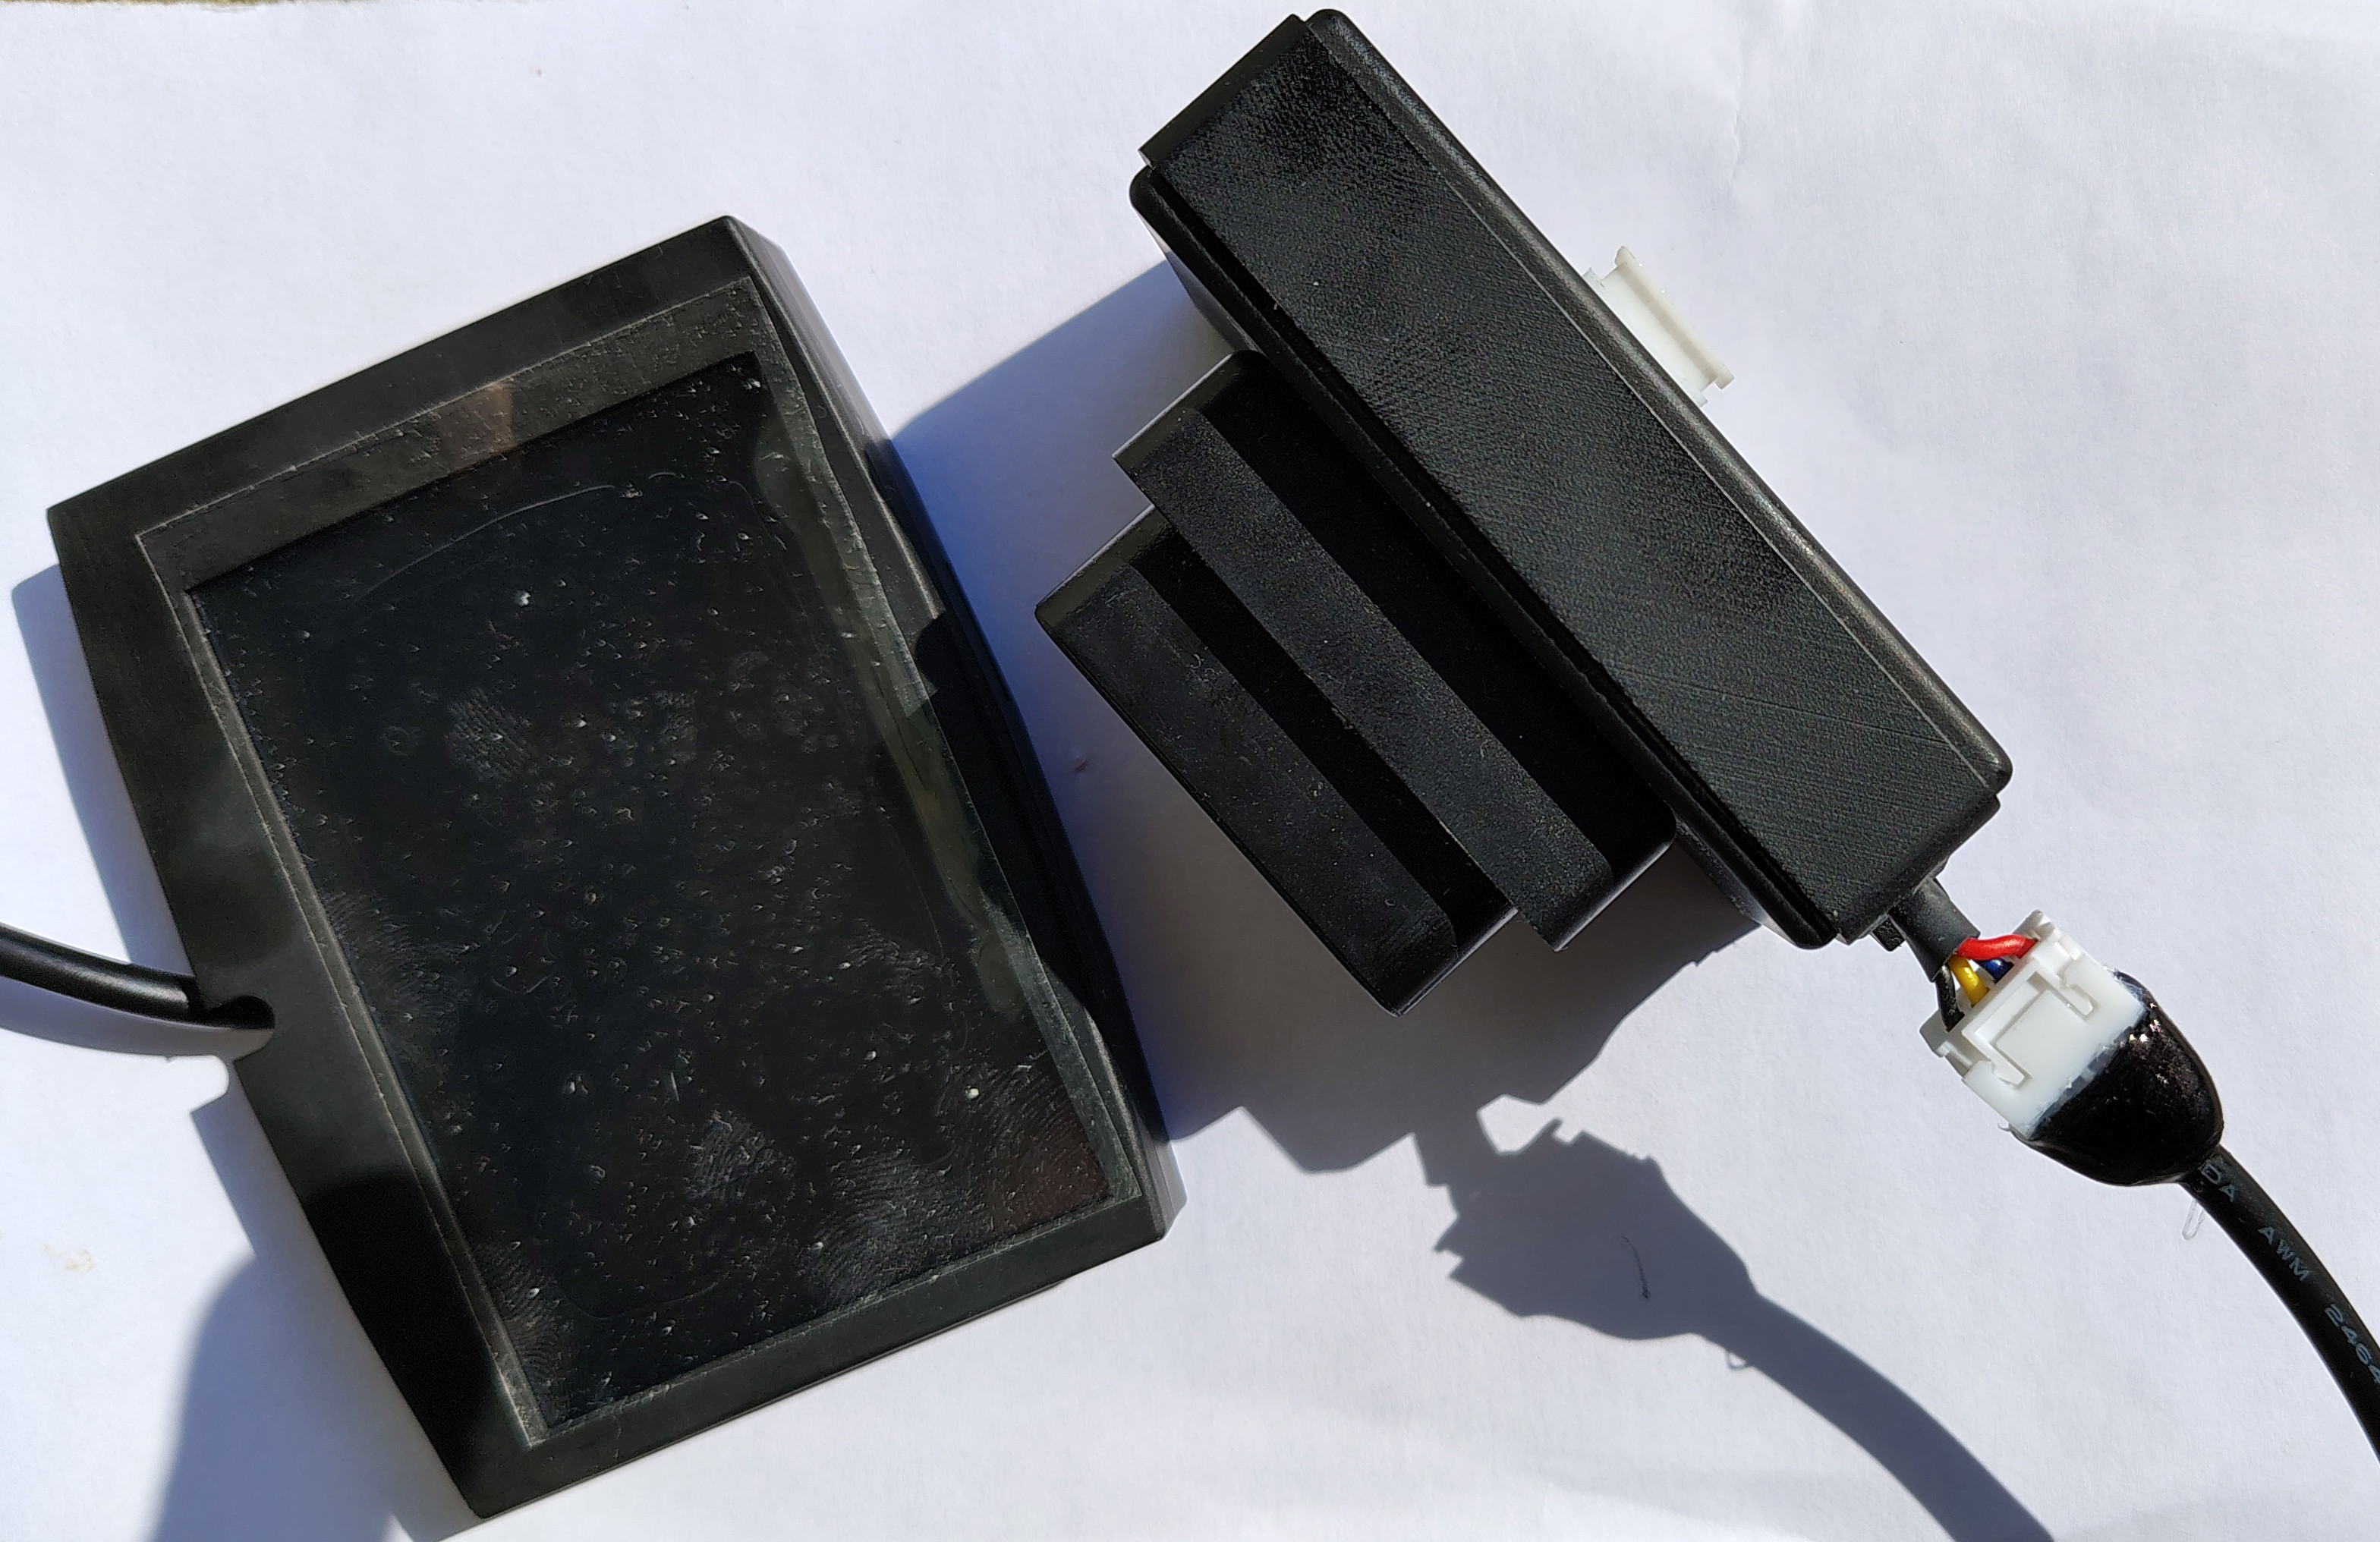
\includegraphics[width=0.8\textwidth]{figures/bb_connection.jpg}
    \caption{Black box connection}
\end{figure}

\section{Black box position}

After you have decided where to place the display, you need to plug in the black box.

The black box needs to be connected to the car's OBD2 port, which is located inside the
left glove box of the Twizy. If you've never opened it before, you will find a small plastic
cover that you need to remove to access the OBD2 port. Once you have access, simply plug in 
the black box and make sure it is securely connected. It only fits in one way, so make sure to align the connector properly before plugging it in.

\begin{figure}[H]
    \centering
    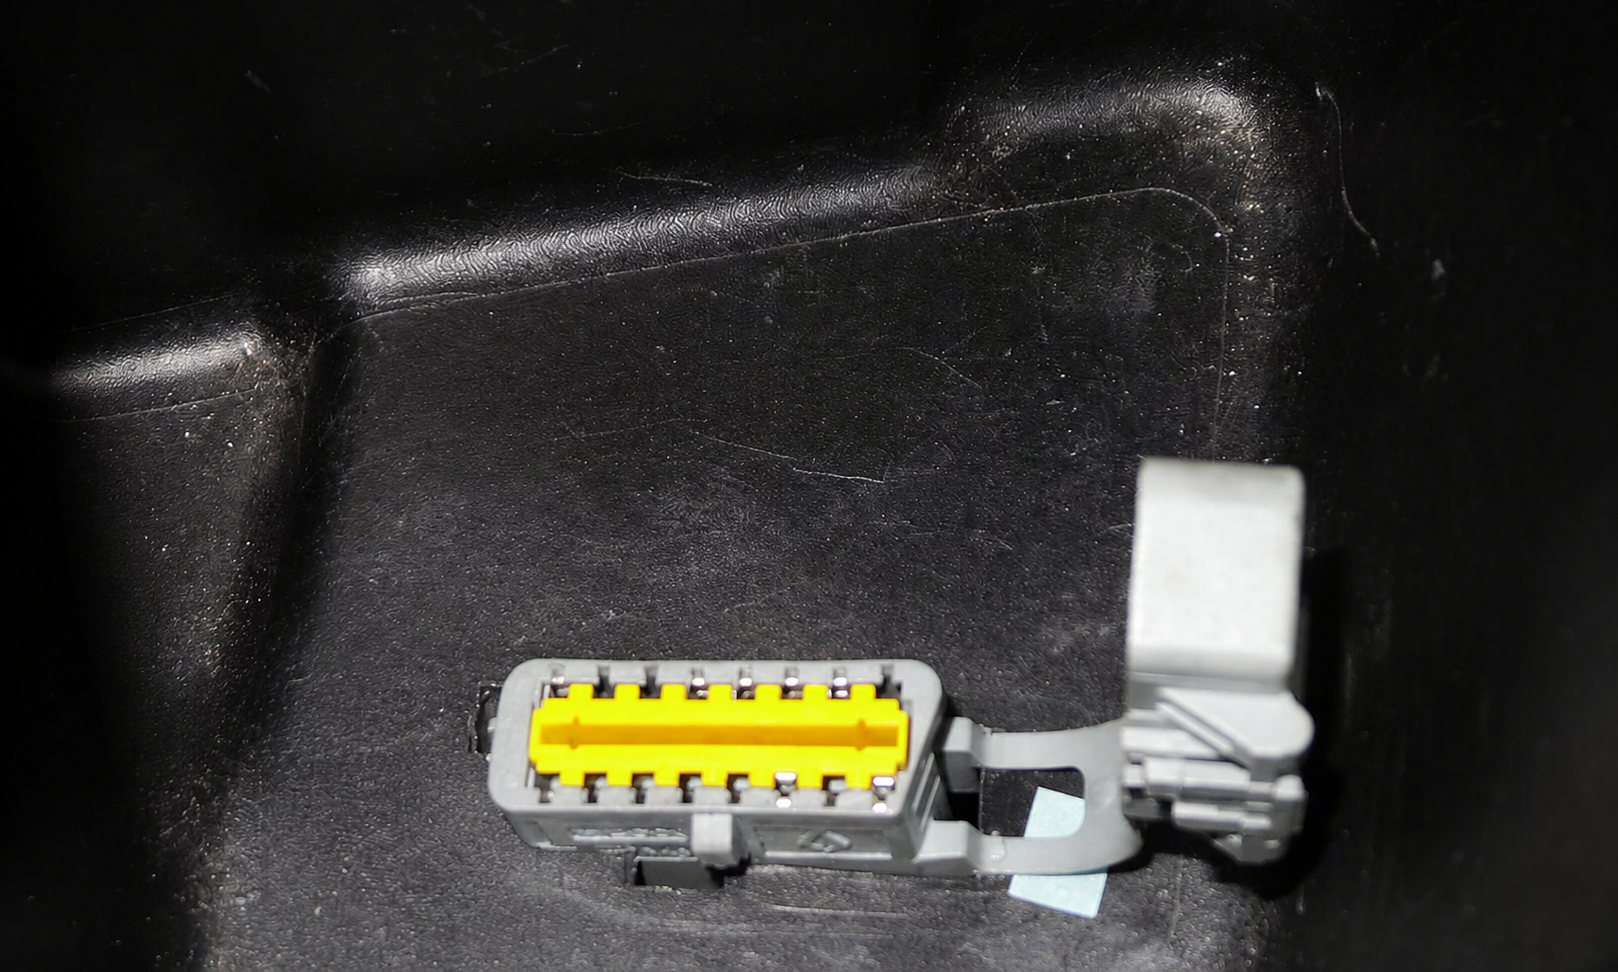
\includegraphics[width=0.8\textwidth]{figures/obd_connector.png}
    \caption{OBD2 connector location in the Twizy}
\end{figure}

\textbf{Only after connecting the display} you can enable the switch on the black box.
And the installation is complete! Now you can start your Twizy and enjoy the ToM+ features.


\section{Wiper stalk button position}

Now it's time to install, if provided, the wiper stalk button to control ToM+ or
BigToM without having to use the touch screen. Just to be clear this button is
shown in Figure~\ref{fig:wiper_stalk_button} and must be connected to the plug
next to the black box switch as highlighted in Figure~\ref{fig:blackbox_components} and below.\\

\begin{figure}[H]
    \centering
    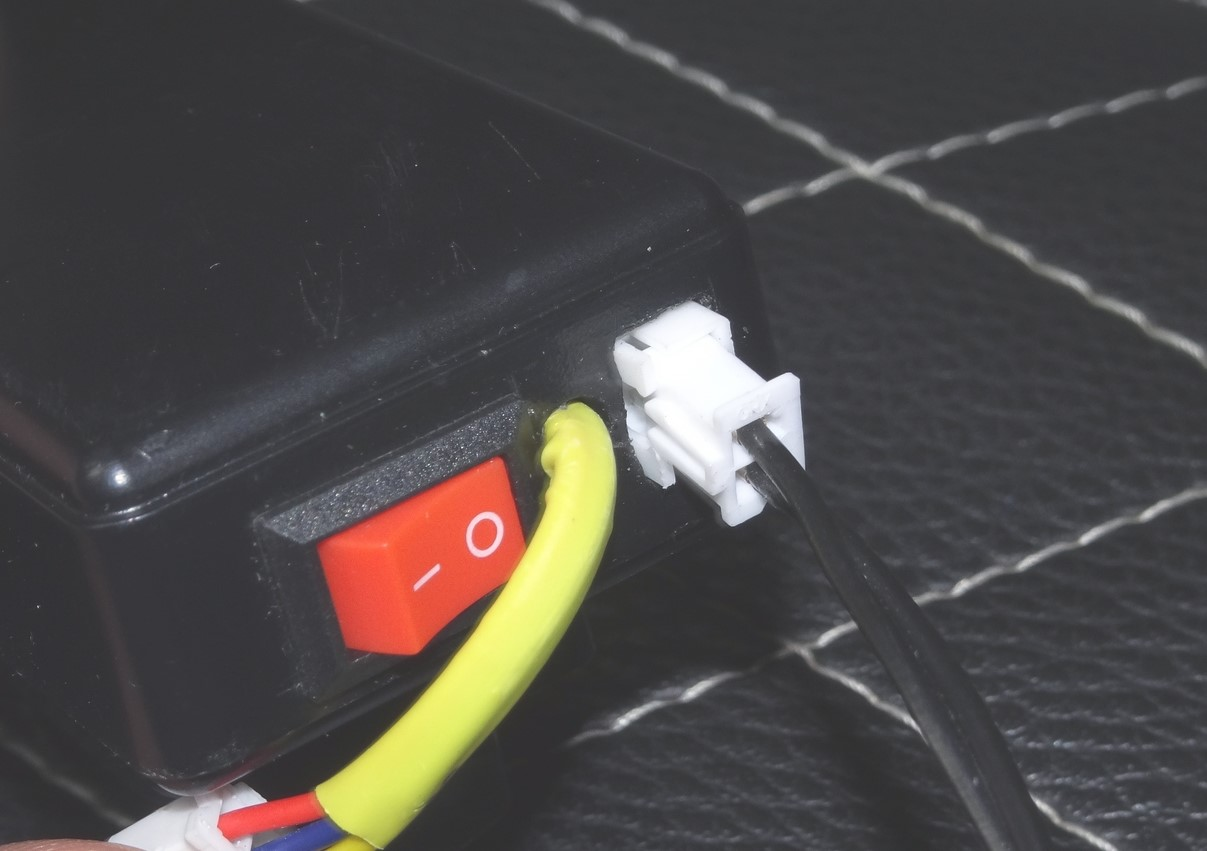
\includegraphics[width=0.7\textwidth]{figures/ButtonConnector.JPG}
    \caption{Black box wiper stalk button connection.}
\end{figure}

To fix and secure the button to the wiper stalk (I personally suggest using it
on the right one), you will need a cable zip tie, provided in the received kit as shown
in Figure~\ref{fig:cable_tie}.

\begin{figure}[H]
    \centering
    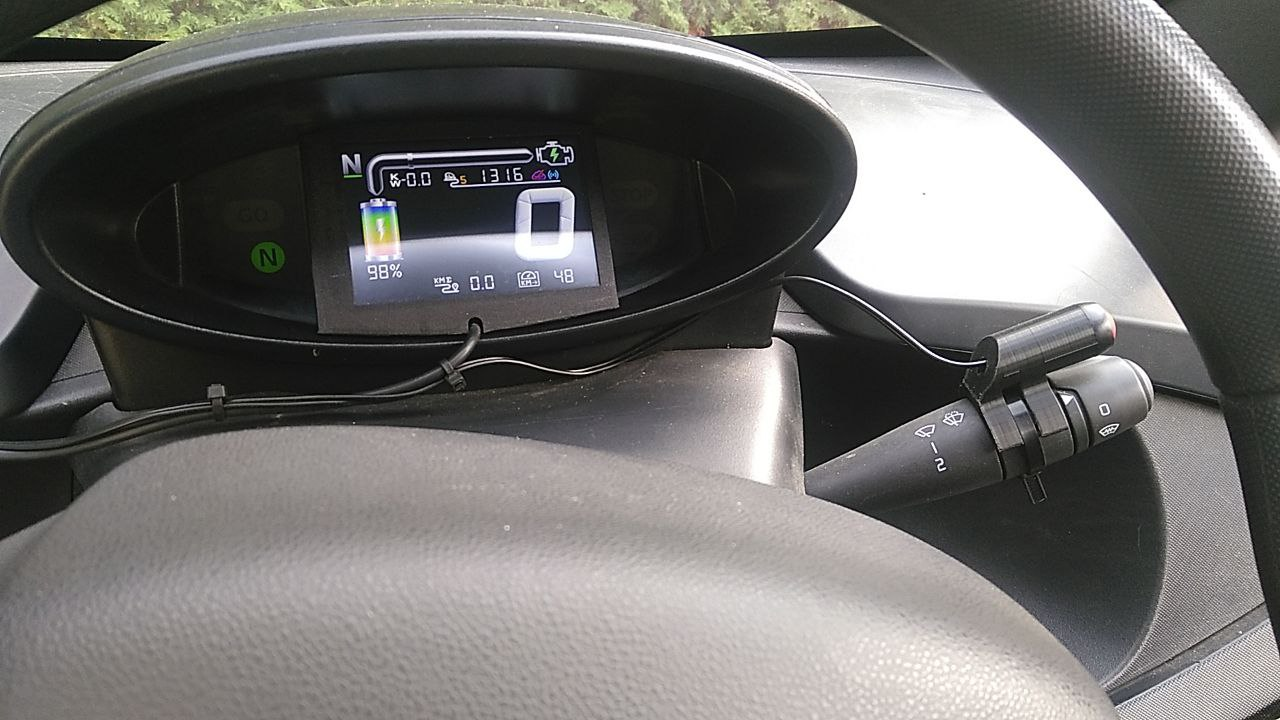
\includegraphics[width=0.8\textwidth]{figures/button_installed.jpg}
    \caption{Wiper stalk button position.}
\end{figure}

To know how to use the wiper stalk button refer to Section~\ref{sec:web_wiper_stalk},
where it's also explained how to customize button presses and performed actions.


\section{Twin ToM --- Secondary display installation}

The Twin ToM was designed for original \textbf{standard ToM owners} to find a new use for
the smaller LCD display as an auxilliary screen. The two displays work simoultaneously
with the same black box and you can monitor different pages at the same time. If
you are a ToM+ owner, you can ask for the smaller display and have an auxilliary
display too.\\

The suggested usage is having the dashboard page on the bigger display (because
this page is not available on the smaller one) and any other page on the standard
ToM display, for instance to monitor motor data.\\

This will work with the original black box version, by updating to the latest
firmware version only. To connect both displays instead, you will need an USB
switch adapter that looks like the one in the image below. To have the \textbf{Twin 
ToM} just email me and ask for the upgrade and you will receive
the bigger ToM+ display along with the shown adapter.

\begin{figure}[H]
    \centering
    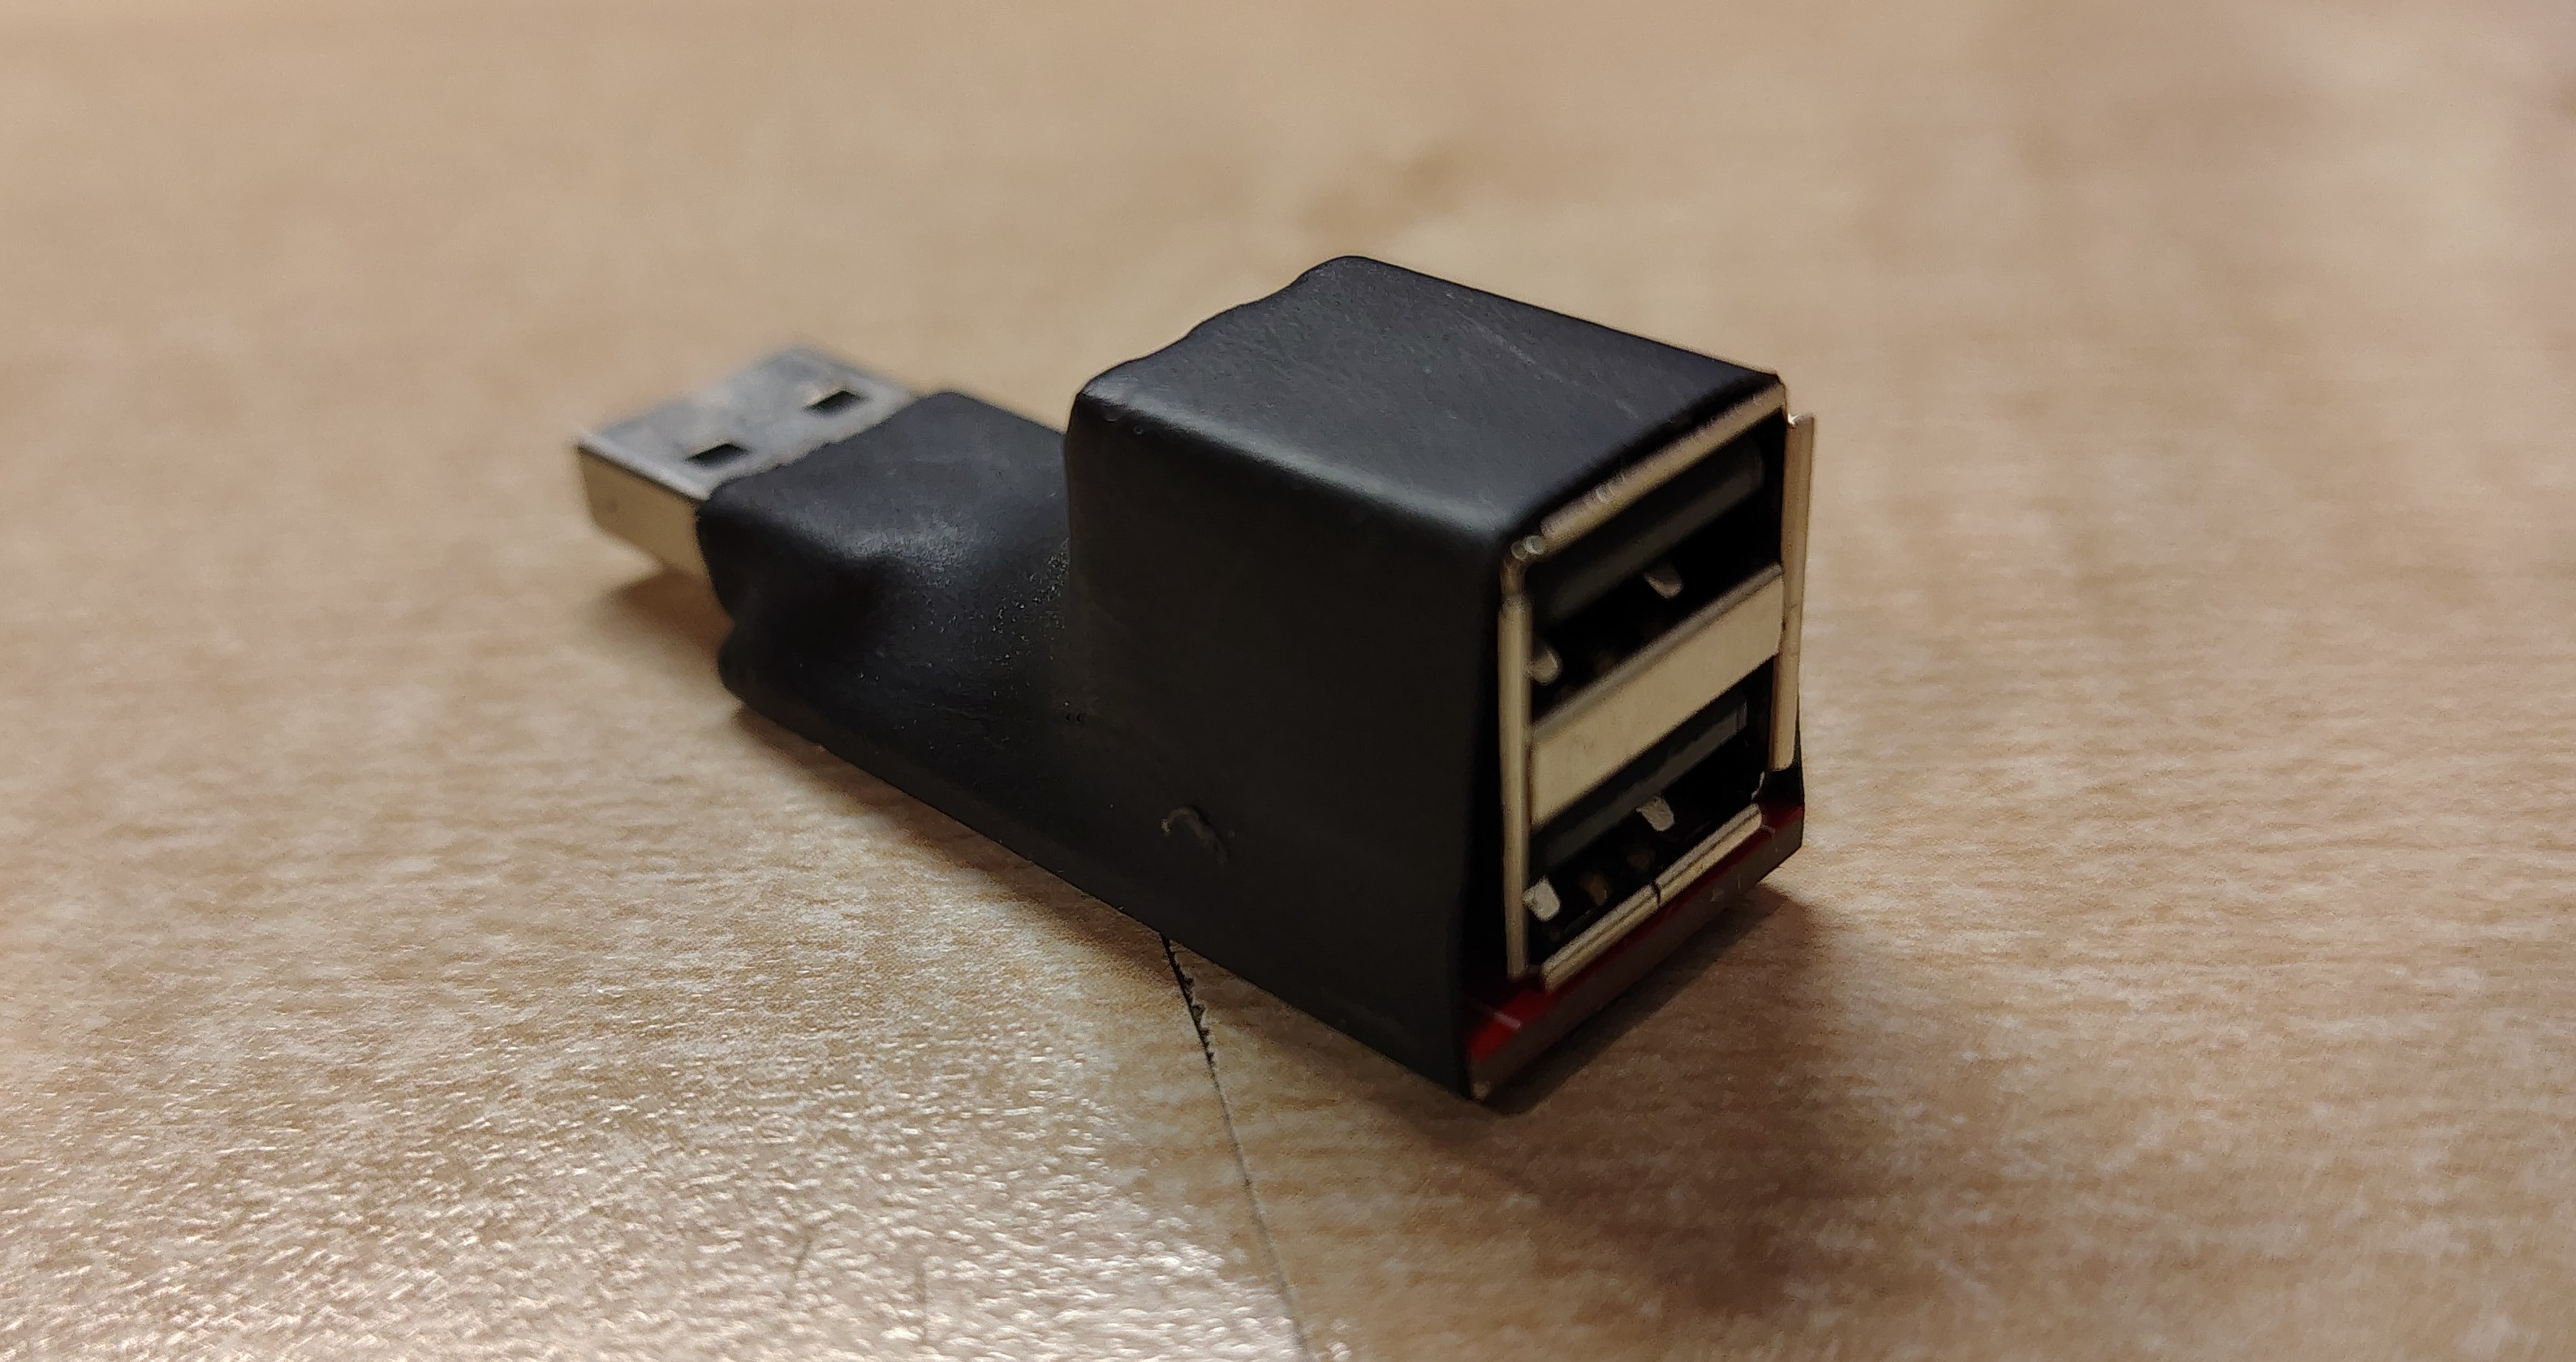
\includegraphics[width=0.7\textwidth]{figures/twintom_adapter.jpg}
    \caption{Twin ToM double USB provided adapter.}
\end{figure}

As already mentioned, Twin ToM is compatible with ToM+ but it requires a different
adapter, than you will receive along with the smaller auxilliary display if you
contact me via email at \textbf{info.twizometer@gmail.com}.